\newpage
\section{Experimentos y Análisis de Resultados}
\label{sec:experimentos}

\subsection{Configuración Experimental y Parámetros}

Para evitar redundancias, se remite al Punto \ref{sec:formulacion} para la definición formal del problema, los conjuntos de datos (IBEX 35, S\&P 100 y S\&P 500) y las restricciones sobre las posiciones de los activos. A continuación se especifican los detalles experimentales necesarios para la reproducibilidad y la comparación empírica.

\subsubsection*{Condiciones de ejecución}

\begin{itemize}
    \item \textbf{Ejecuciones independientes:} 50 por algoritmo y mercado. Semilla base $seed=42$, incrementada secuencialmente ($42+i$).
    \item \textbf{Criterio de parada global:} máximo de 10\,000 evaluaciones de la función objetivo para todos los algoritmos estocásticos.
    \item \textbf{Datos y partición temporal:} fase de búsqueda de optimización en el periodo 2015--2024 y fase de prueba de dicha optimización en el periodo 2025 para todos los algoritmos.
\end{itemize}

\subsubsection*{Parámetros de los algoritmos de trayectoria}

\begin{itemize}
    \item \textbf{Enfriamiento Simulado:} $\mu=0.2$, $\phi=0.3$, $T_f=10^{-3}$, $max\_vecinos=10 \cdot n$ y $max\_exitos = n$ (equivalente a $0.1\cdot max\_vecinos$).
    \item \textbf{BMB e ILS:} 5 arranques por ejecución. La BL interna se acota a 2000 evaluaciones por arranque.
    \item \textbf{ILS:} tasa de mutación del 20\% para la perturbación de la mejor solución.
    \item \textbf{ILS-ES:} misma perturbación que ILS, sustituyendo la BL por ES en cada arranque.
\end{itemize}

\subsubsection*{Parámetros de la búsqueda local en el algoritmo de referencia (P2)}

El mejor algoritmo de la Práctica 2 identificado en las ejecuciones es \textbf{AM-Best}. Se mantiene como referencia en tablas y análisis con los parámetros configurados en \texttt{config.cfg}:

\begin{itemize}
    \item \textbf{Frecuencia:} cada 10 generaciones.
    \item \textbf{Aplicación:} BL aplicada al 10\% superior (AM-Best).
    \item \textbf{Intensidad:} máximo 100 evaluaciones por BL; ratio de transferencia reducido al 15\%.
\end{itemize}

\subsection{Resultados Numéricos y Boxplots}

Se muestran las tablas exigidas por el guion, incluyendo Greedy, Random y BL (P1), el mejor algoritmo de P2 (AM-Best), y las técnicas de trayectoria de P3 (BMB, ILS, ES, ILS-ES). Los valores provienen de la salida de ejecución en \texttt{salida.txt}.

\begin{table}[H]
\centering
\caption{Resultados numéricos -- IBEX 35}
\label{tab:global-ibex35}
\resizebox{\textwidth}{!}{%
\begin{tabular}{lcccccc}
\hline
Algoritmo & Fitness(2015--2024) & Fitness(2025) & Beneficio(2025) & Std & Evaluaciones & Tiempo (s) \\
\hline
Greedy & -4.794 & -3.227 & -0.033 & 0.000 & 1 & 0.000 \\
Random & -4.911 & -3.305 & 0.052 & 0.091 & 10000 & 0.025 \\
BL & -4.614 & -3.116 & 0.021 & 0.039 & 1078 & 0.001 \\
Mejor P2 (AM-Best) & -4.490 & -3.083 & 0.033 & 0.000 & 10000 & 0.007 \\
BMB & -4.574 & -3.107 & 0.023 & 0.020 & 5403 & 0.004 \\
ILS & -4.606 & -3.115 & 0.021 & 0.036 & 4349 & 0.003 \\
ES & -4.653 & -3.126 & 0.020 & 0.010 & 3244 & 0.002 \\
ILS-ES & -4.649 & -3.127 & 0.020 & 0.014 & 3130 & 0.002 \\
\hline
\end{tabular}
}
\end{table}

\begin{table}[H]
\centering
\caption{Resultados numéricos -- S\&P 100}
\label{tab:global-sp100}
\resizebox{\textwidth}{!}{%
\begin{tabular}{lcccccc}
\hline
Algoritmo & Fitness(2015--2024) & Fitness(2025) & Beneficio(2025) & Std & Evaluaciones & Tiempo (s) \\
\hline
Greedy & -3.305 & -3.791 & 0.100 & 0.000 & 1 & 0.000 \\
Random & -3.400 & -4.080 & 0.079 & 0.041 & 10000 & 0.069 \\
BL & -3.116 & -3.890 & 0.097 & 0.084 & 4351 & 0.023 \\
Mejor P2 (AM-Best) & -2.816 & -3.734 & 0.100 & 0.008 & 10000 & 0.036 \\
BMB & -3.006 & -3.863 & 0.092 & 0.046 & 10000 & 0.065 \\
ILS & -3.114 & -3.888 & 0.097 & 0.082 & 9926 & 0.055 \\
ES & -3.300 & -3.987 & 0.088 & 0.030 & 1828 & 0.011 \\
ILS-ES & -3.311 & -3.991 & 0.085 & 0.038 & 2863 & 0.017 \\
\hline
\end{tabular}
}
\end{table}

\begin{table}[H]
\centering
\caption{Resultados numéricos -- S\&P 500}
\label{tab:global-sp500}
\resizebox{\textwidth}{!}{%
\begin{tabular}{lcccccc}
\hline
Algoritmo & Fitness(2015--2024) & Fitness(2025) & Beneficio(2025) & Std & Evaluaciones & Tiempo (s) \\
\hline
Greedy & -3.370 & -3.909 & 0.024 & 0.000 & 1 & 0.000 \\
Random & -3.648 & -4.364 & 0.019 & 0.044 & 10000 & 0.678 \\
BL & -3.428 & -4.330 & 0.004 & 0.154 & 9645 & 0.603 \\
Mejor P2 (AM-Best) & -2.735 & -3.898 & 0.017 & 0.037 & 10000 & 0.367 \\
BMB & -3.263 & -4.189 & 0.010 & 0.078 & 10000 & 1.071 \\
ILS & -3.434 & -4.312 & 0.005 & 0.146 & 10000 & 0.689 \\
ES & -4.062 & -4.760 & 0.010 & 0.101 & 308 & 0.016 \\
ILS-ES & -4.035 & -4.761 & 0.007 & 0.092 & 546 & 0.030 \\
\hline
\end{tabular}
}
\end{table}

A continuación se presentan los boxplots correspondientes a los algoritmos de la Práctica 3 para cada mercado:

\begin{figure}[H]
\centering
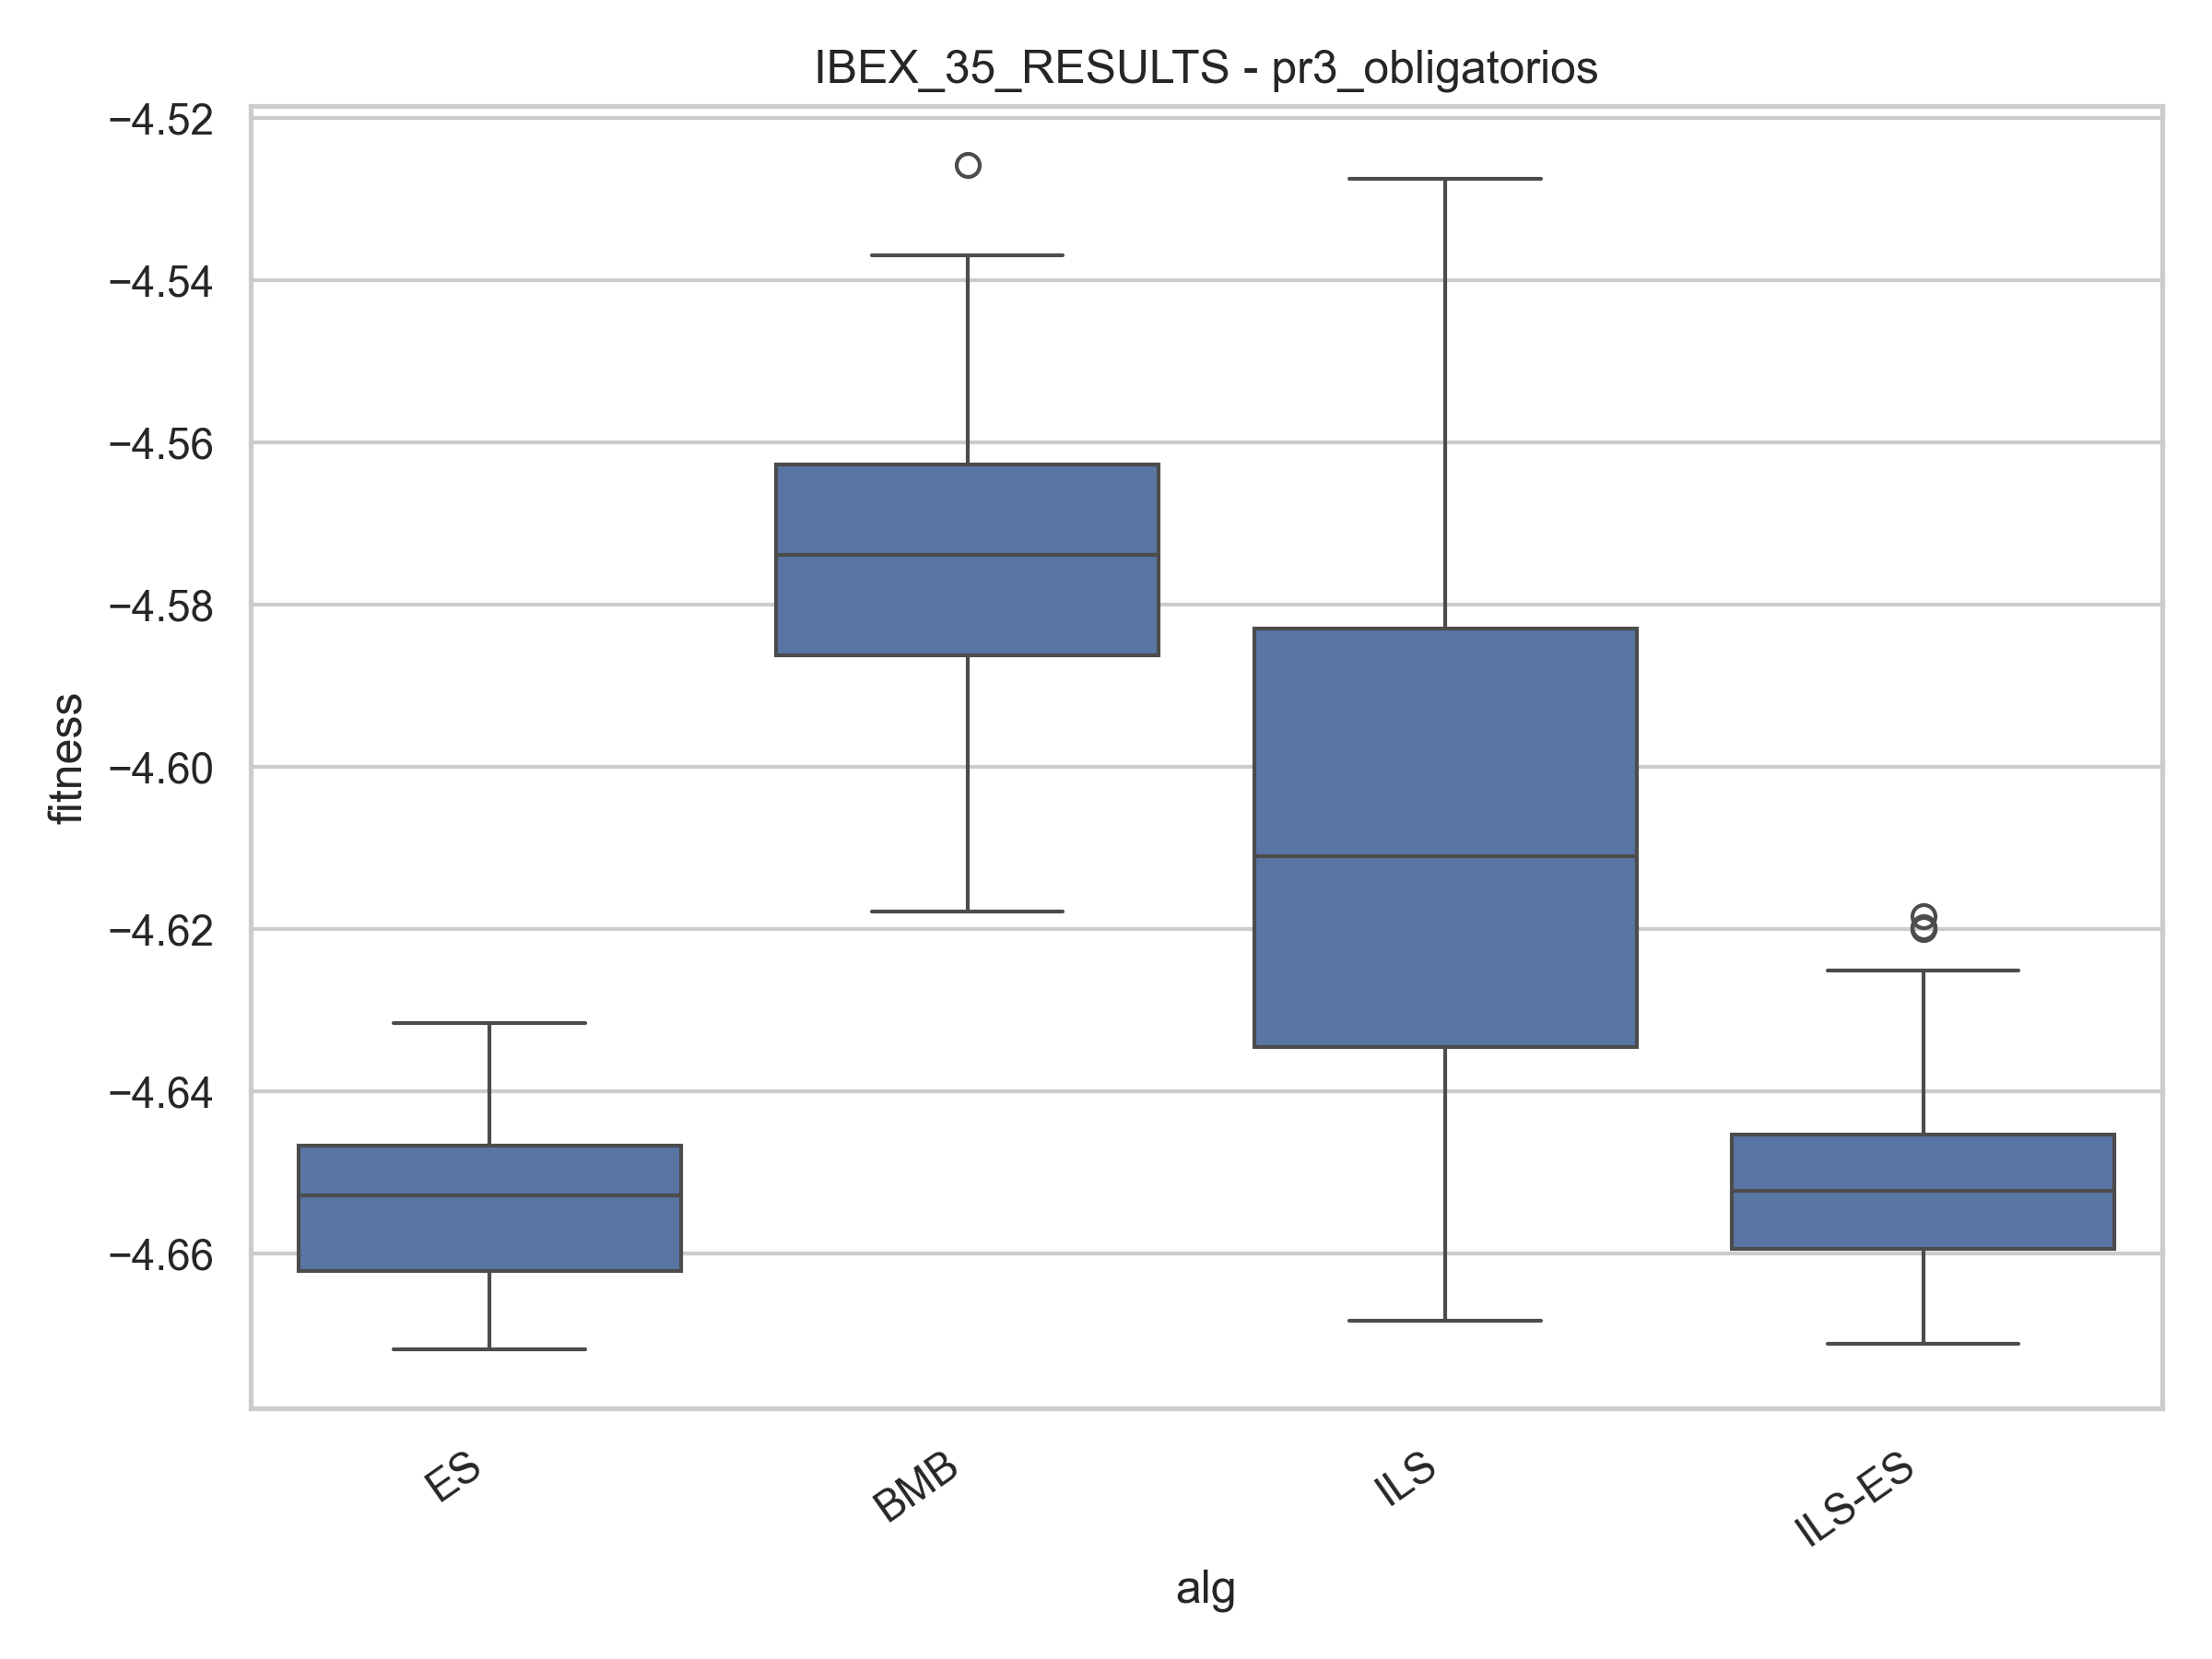
\includegraphics[width=0.8\textwidth]{figuras/IBEX_35_RESULTS_pr3_obligatorios.png}
\caption{Boxplots algoritmos trayectoria (Práctica 3) -- IBEX 35.}
\label{fig:pr3-obligatorios-ibex}
\end{figure}

\begin{figure}[H]
\centering

\includegraphics[width=0.8\textwidth]{\detokenize{figuras/S&P_100_RESULTS_pr3_obligatorios.png}}
\caption{Boxplots algoritmos trayectoria (Práctica 3) -- S\&P 100.}
\label{fig:pr3-obligatorios-sp100}
\end{figure}

\begin{figure}[H]
\centering

\includegraphics[width=0.8\textwidth]{\detokenize{figuras/S&P_500_RESULTS_pr3_obligatorios.png}}
\caption{Boxplots algoritmos trayectoria (Práctica 3) -- S\&P 500.}
\label{fig:pr3-obligatorios-sp500}
\end{figure}

\subsection{Análisis de Resultados}

El guion exige comparar algoritmos \textbf{similares} para aislar el elemento diferenciador.
La Figura~\ref{fig:heatmap-mejora} sintetiza en términos porcentuales la mejora (o empeoramiento)
de cada algoritmo respecto a la Búsqueda Local (BL), que actúa como referencia de partida.

\begin{figure}[H]
\centering
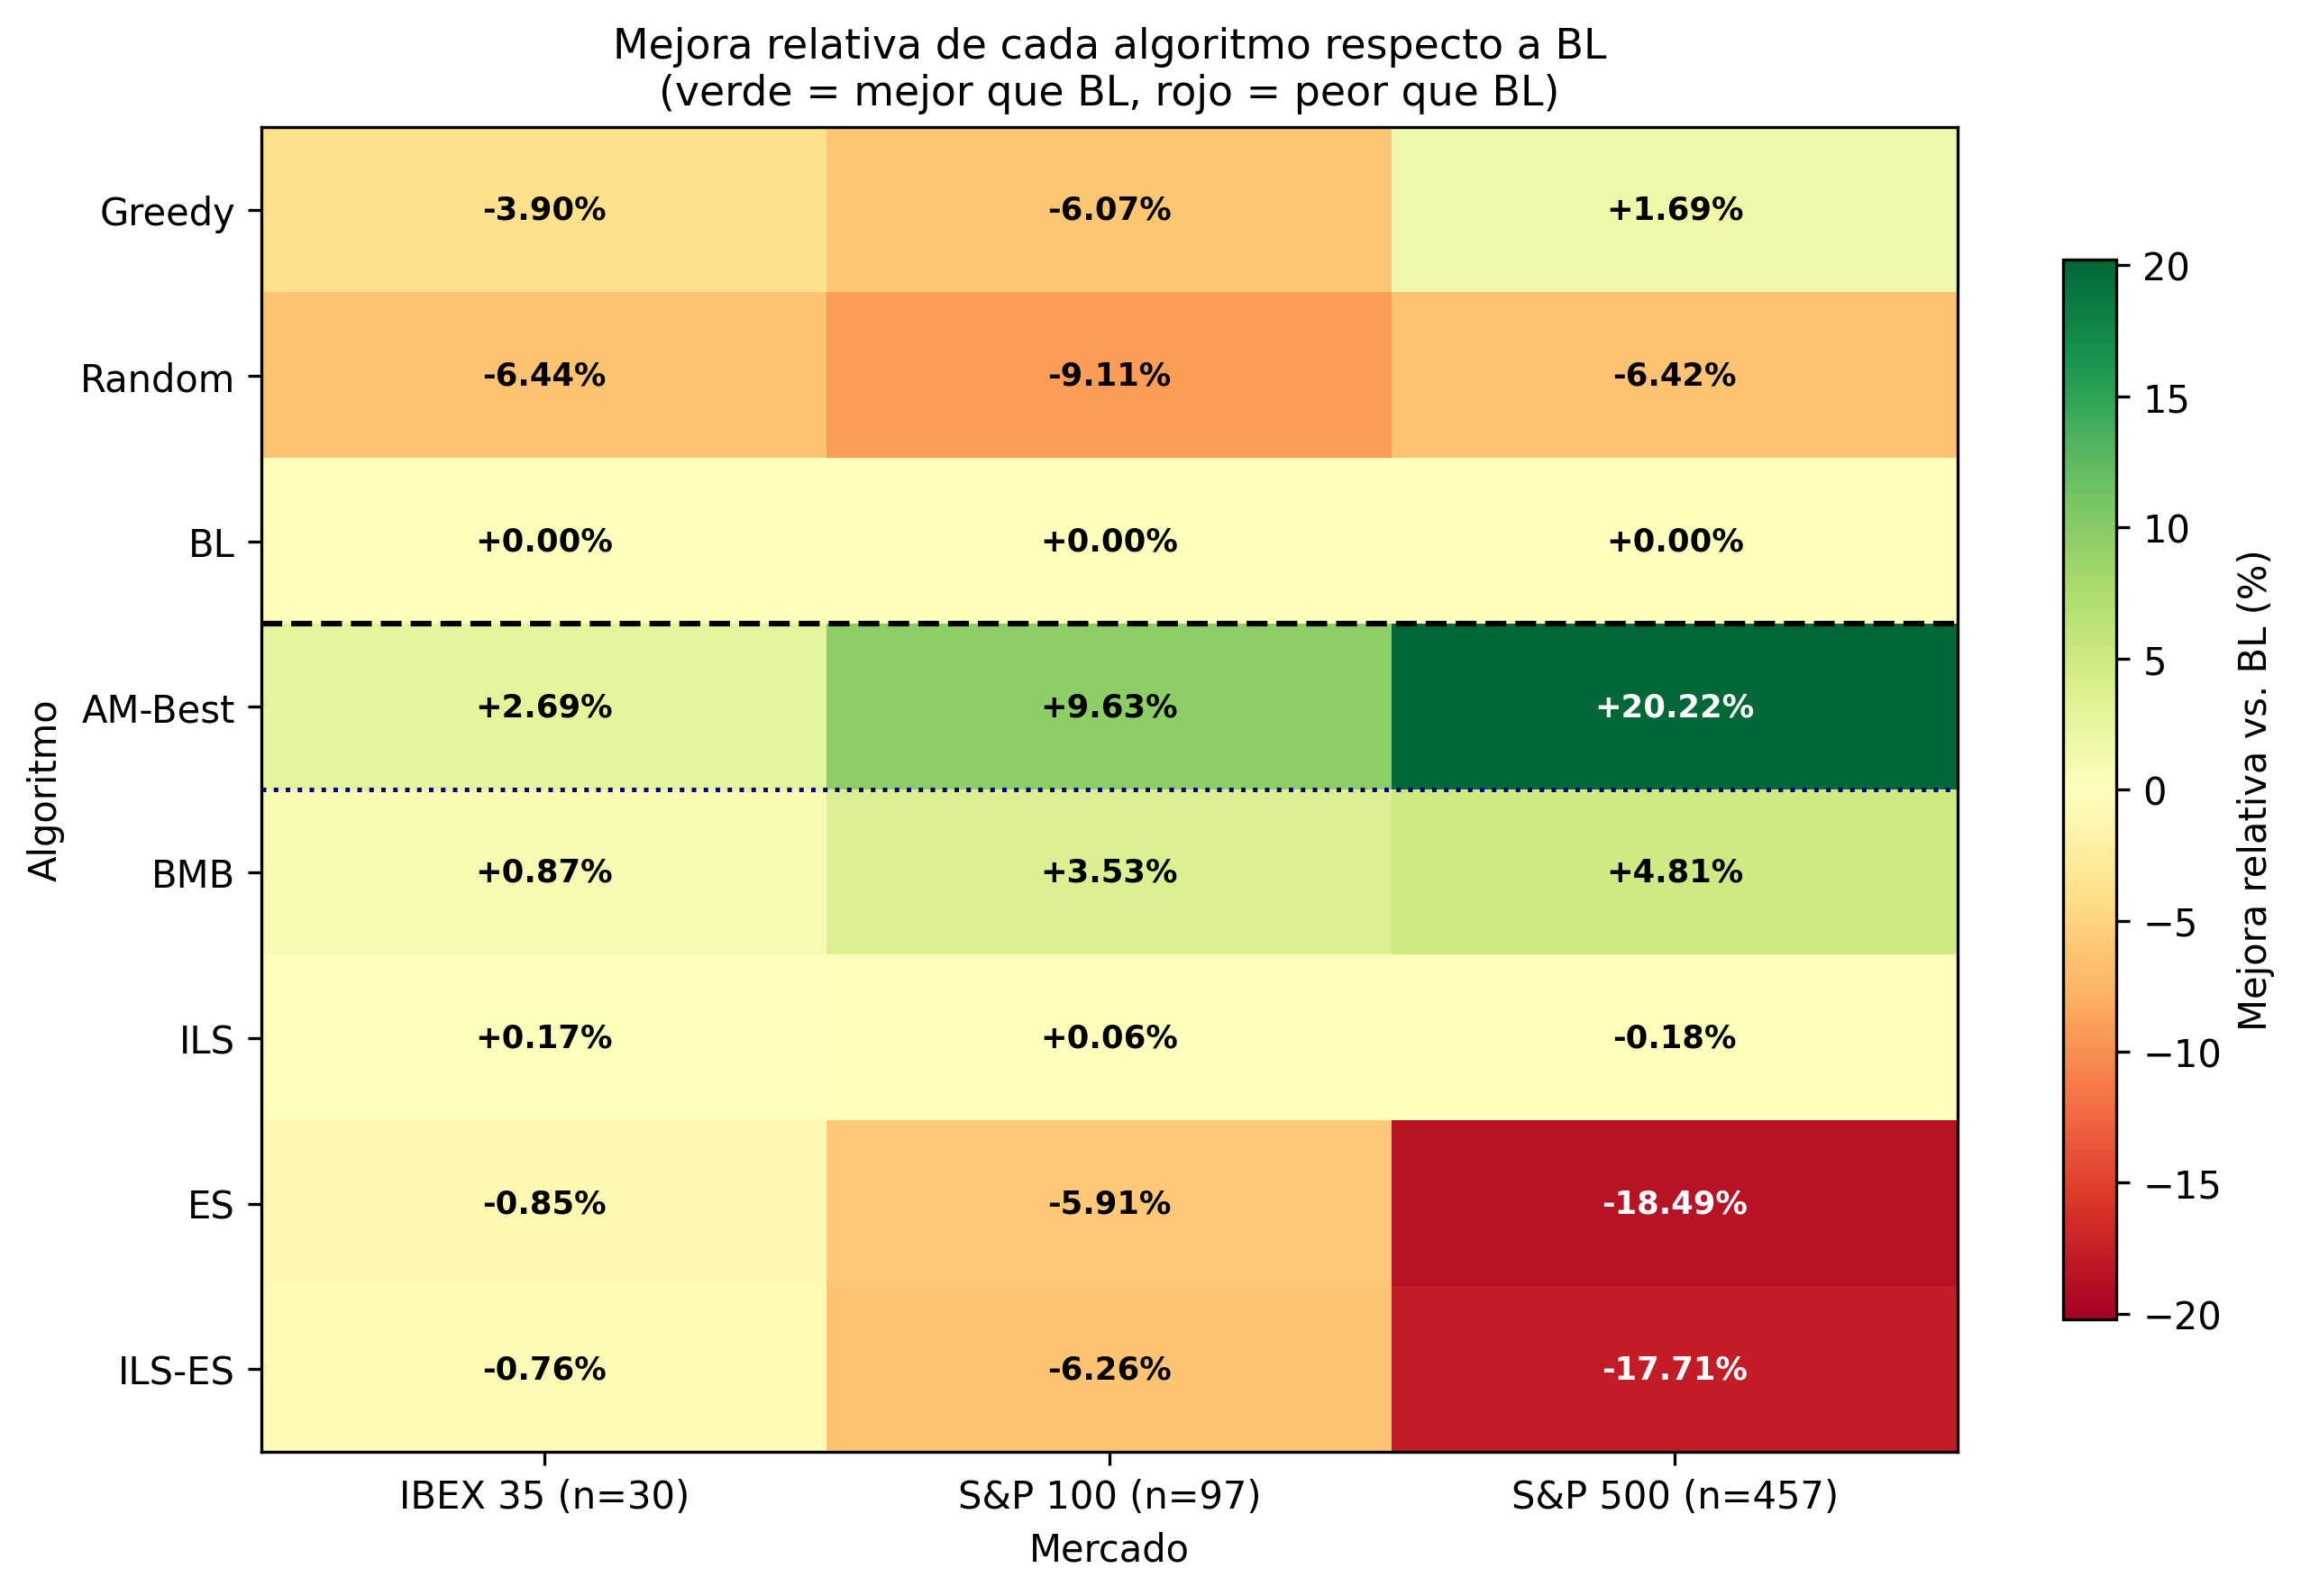
\includegraphics[width=\textwidth]{figuras/heatmap_mejora_vs_bl.png}
\caption{Mejora relativa porcentual de cada algoritmo respecto a BL.
Verde = supera a BL; rojo = peor que BL.}
\label{fig:heatmap-mejora}
\end{figure}

\subsubsection*{BL frente a las técnicas de trayectoria (BMB, ILS, ES, ILS-ES)}

La Búsqueda Local constituye el bloque base de todos los algoritmos de trayectoria de la P3:
BMB e ILS la invocan repetidamente, mientras que ES la reemplaza por exploración estocástica.
El heatmap (Figura~\ref{fig:heatmap-mejora}) muestra que \textbf{BMB mejora a BL en un
0.87\,\% en IBEX 35 y un 3.54\,\% en S\&P 100}, pero no consigue superarla en S\&P 500
($-4.8\,\%$). Esto se explica por el comportamiento de la BL en alta dimensión: con
presupuesto total de 10\,000 evaluaciones y 5 arranques de 2000 cada uno, BMB explora bien
cuencas diferentes en problemas pequeños, pero en S\&P 500 (457 activos) cada arranque de 2000
evaluaciones es insuficiente para que la BL interna converja a un óptimo de calidad.

\textbf{ILS}, a diferencia de BMB, reutiliza la mejor solución mediante perturbación del 20\,\%.
En IBEX 35 obtiene un resultado cercano a BL ($-0.26\,\%$ respecto a ella), y en S\&P 100
prácticamente la iguala ($-0.06\,\%$). La perturbación del ILS, al barajar el 20\,\% de los
pesos, no introduce suficiente diversidad en espacios de alta dimensión, por lo que la búsqueda
reincide en cuencas similares a la del mejor actual: ILS actúa de forma más explotadora que BMB.

\textbf{ES} obtiene resultados peores que BL en los tres mercados ($-0.84\,\%$ en IBEX 35,
$-5.9\,\%$ en S\&P 100, $-18.5\,\%$ en S\&P 500). Esto responde a una razón estructural: con
$\max\_vecinos = 10n$ y solo $\approx 308$ evaluaciones en S\&P 500, el ES realiza muy pocos
ciclos de enfriamiento antes de agotar el presupuesto, sin llegar a explotar el espacio de forma
efectiva. Sin embargo, su \textbf{coste es drásticamente menor} (véase la Figura~\ref{fig:scatter-tradeoff}),
lo que lo convierte en la opción más eficiente en tiempo por unidad de calidad en problemas pequeños.

\subsubsection*{BMB frente a ILS: reinicio ciego vs. reinicio informado}

Ambos algoritmos comparten exactamente la misma estructura (5 arranques de BL con 2000 evaluaciones),
con una única diferencia: \textbf{BMB genera el punto de partida de forma aleatoria}, mientras que
\textbf{ILS muta la mejor solución encontrada}. La diferencia de fitness media en IBEX 35 es del
$0.70\,\%$ a favor de BMB, y en S\&P 100 del $2.9\,\%$. Este resultado, aparentemente contraintuitivo,
se justifica porque la perturbación del 20\,\% del ILS no es suficientemente disruptiva para escapar de la
cuenca del mejor actual en carteras de muchos activos, haciendo que todos los arranques exploren
la misma zona del espacio. El reinicio completamente aleatorio de BMB, en cambio, garantiza la
cobertura de cuencas diversas en cada arranque.

\subsubsection*{ES frente a ILS-ES: impacto de sustituir BL por ES como motor}

ILS-ES sustituye la BL interna del ILS por un enfriamiento simulado completo. En IBEX 35, ILS-ES
obtiene prácticamente el mismo fitness que ES ($-4.649$ vs. $-4.653$, diferencia del $0.09\,\%$),
pero en S\&P 100 es ligeramente peor ($-3.311$ vs. $-3.300$, diferencia de $0.33\,\%$). La
perturbación ILS no aporta ventaja apreciable sobre ejecutar el ES desde una solución aleatoria,
ya que el ES por sí solo ya explora zonas alejadas del espacio mediante el criterio de Metrópolis.
Esto sugiere que la hibridación ILS-ES es redundante cuando el ES tiene presupuesto suficiente.

\subsubsection*{AM-Best (P2) como referencia superior}

El mejor algoritmo de la P2 (AM-Best) mejora a BL en un \textbf{2.69\,\% en IBEX 35,
9.62\,\% en S\&P 100 y 20.2\,\% en S\&P 500}. La superioridad crece con la dimensión porque
la búsqueda poblacional distribuye las evaluaciones explorando simultáneamente múltiples cuencas.
Con 10\,000 evaluaciones y poblaciones de 50 individuos, AM-Best realiza 200 generaciones con
BL aplicada selectivamente al 10\,\% mejor, combinando exploración y explotación de forma mucho
más efectiva que cualquier algoritmo de trayectoria única.

\subsubsection*{Análisis de outliers}

Los boxplots de las Figuras~\ref{fig:pr3-obligatorios-ibex}--\ref{fig:pr3-obligatorios-sp500}
muestran comportamientos atípicos que conviene justificar teóricamente:
\begin{itemize}[noitemsep]
    \item \textbf{IBEX 35 — outlier superior en BMB:} en una ejecución, el arranque aleatorio
    inicializó en una cuenca de atracción especialmente favorable; al no tener memoria del mejor
    anterior (como sí tiene ILS), ese arranque fue explotado hasta el máximo por la BL interna.
    \item \textbf{IBEX 35 — outliers superiores en ILS-ES:} la combinación del criterio de
    Metrópolis con la perturbación ILS permitió escapar de valles locales en dos ejecuciones
    concretas, saltando a cuencas de mayor calidad que no alcanzó ninguna otra técnica.
    \item \textbf{S\&P 100 — outlier inferior en BMB:} el punto de partida aleatorio cayó en
    una zona extremadamente pobre del espacio, y los 2000 evaluaciones de BL no fueron suficientes
    para escapar de ese valle.
    \item \textbf{S\&P 500 — outlier superior en ES:} en esa ejecución, el esquema de enfriamiento
    Cauchy modificado encontró por aceptación probabilística una cuenca de calidad inhabitual,
    demostrando que el criterio de Metrópolis puede —en ocasiones— superar a la explotación pura
    de BL incluso con muy pocas evaluaciones.
\end{itemize}

\subsection{Estudio de Eficiencia y Trade-off Calidad/Coste}

\begin{figure}[H]
\centering
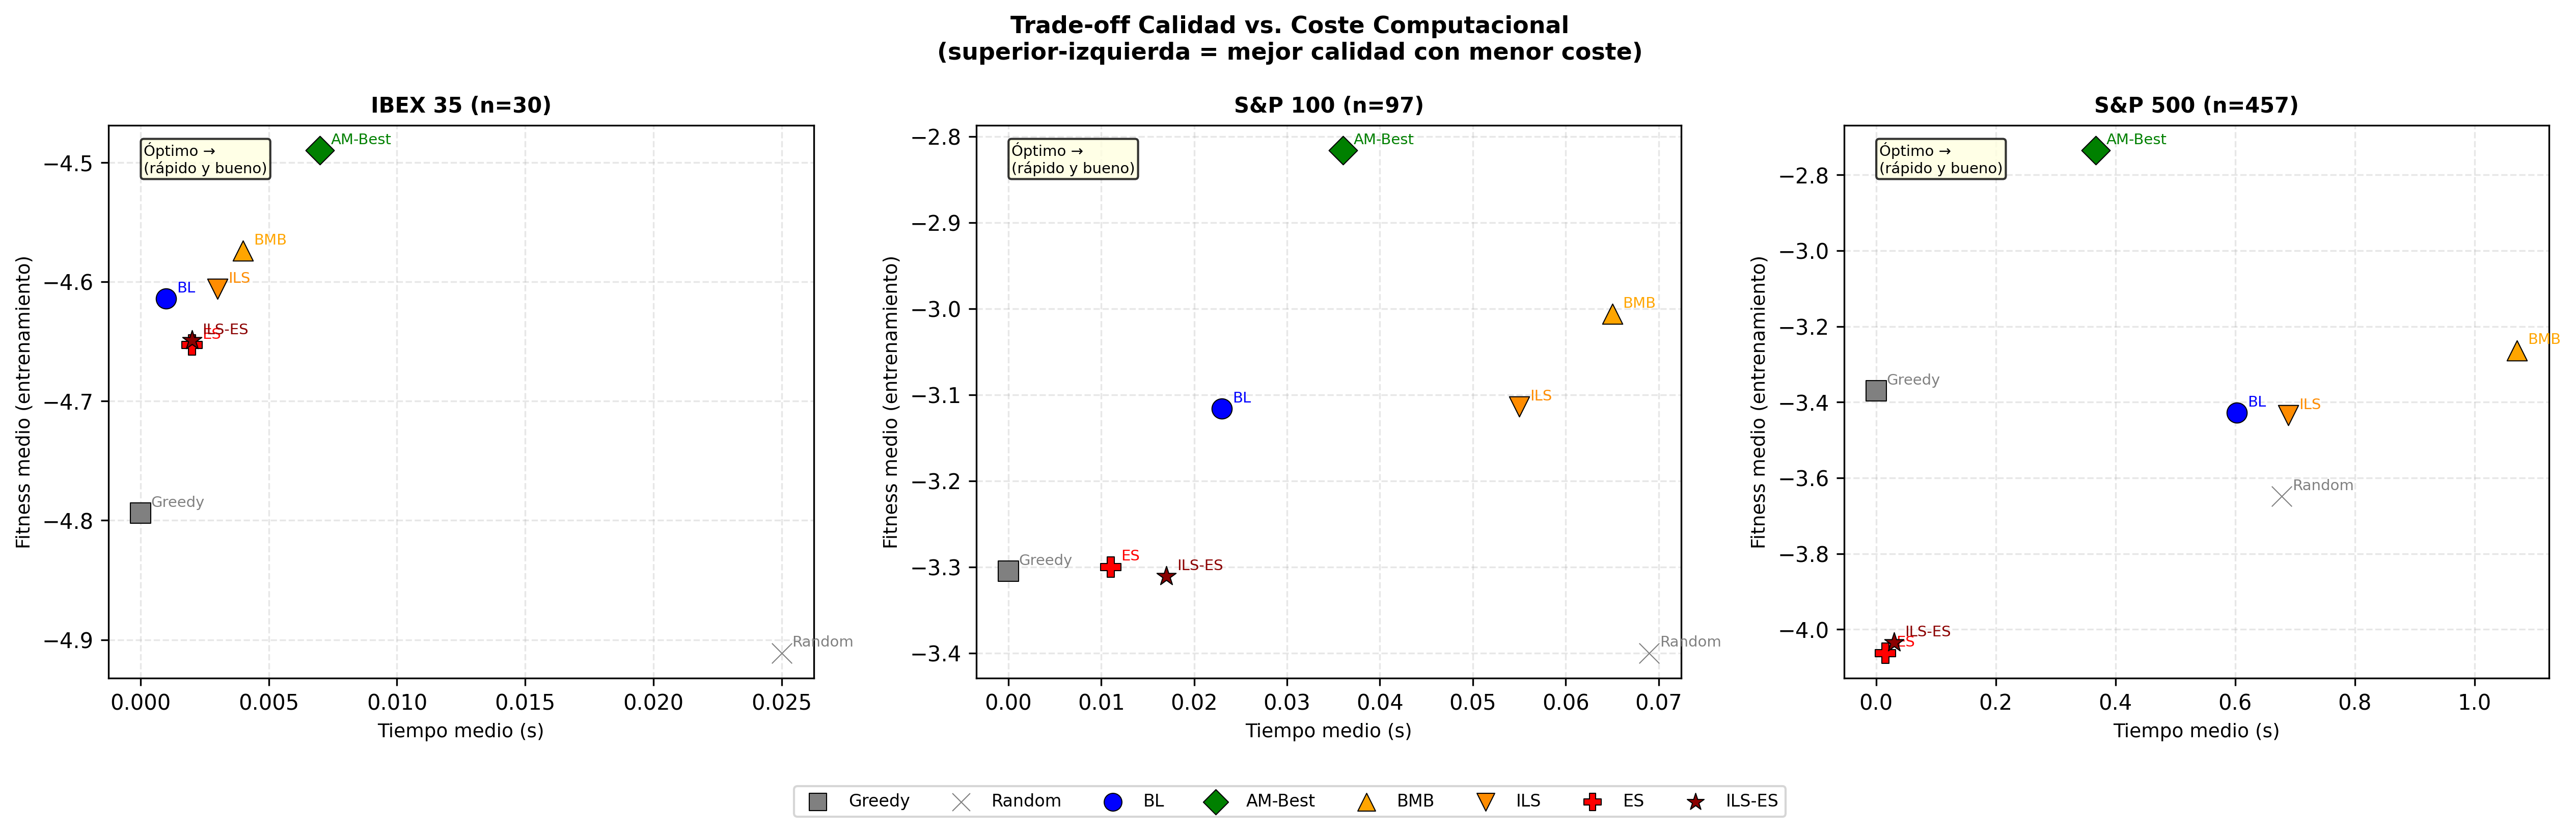
\includegraphics[width=\textwidth]{figuras/scatter_tradeoff_calidad_tiempo.png}
\caption{Trade-off calidad vs.\ coste computacional. Superior-izquierda = mayor calidad
con menor tiempo de ejecución.}
\label{fig:scatter-tradeoff}
\end{figure}

\begin{figure}[H]
\centering
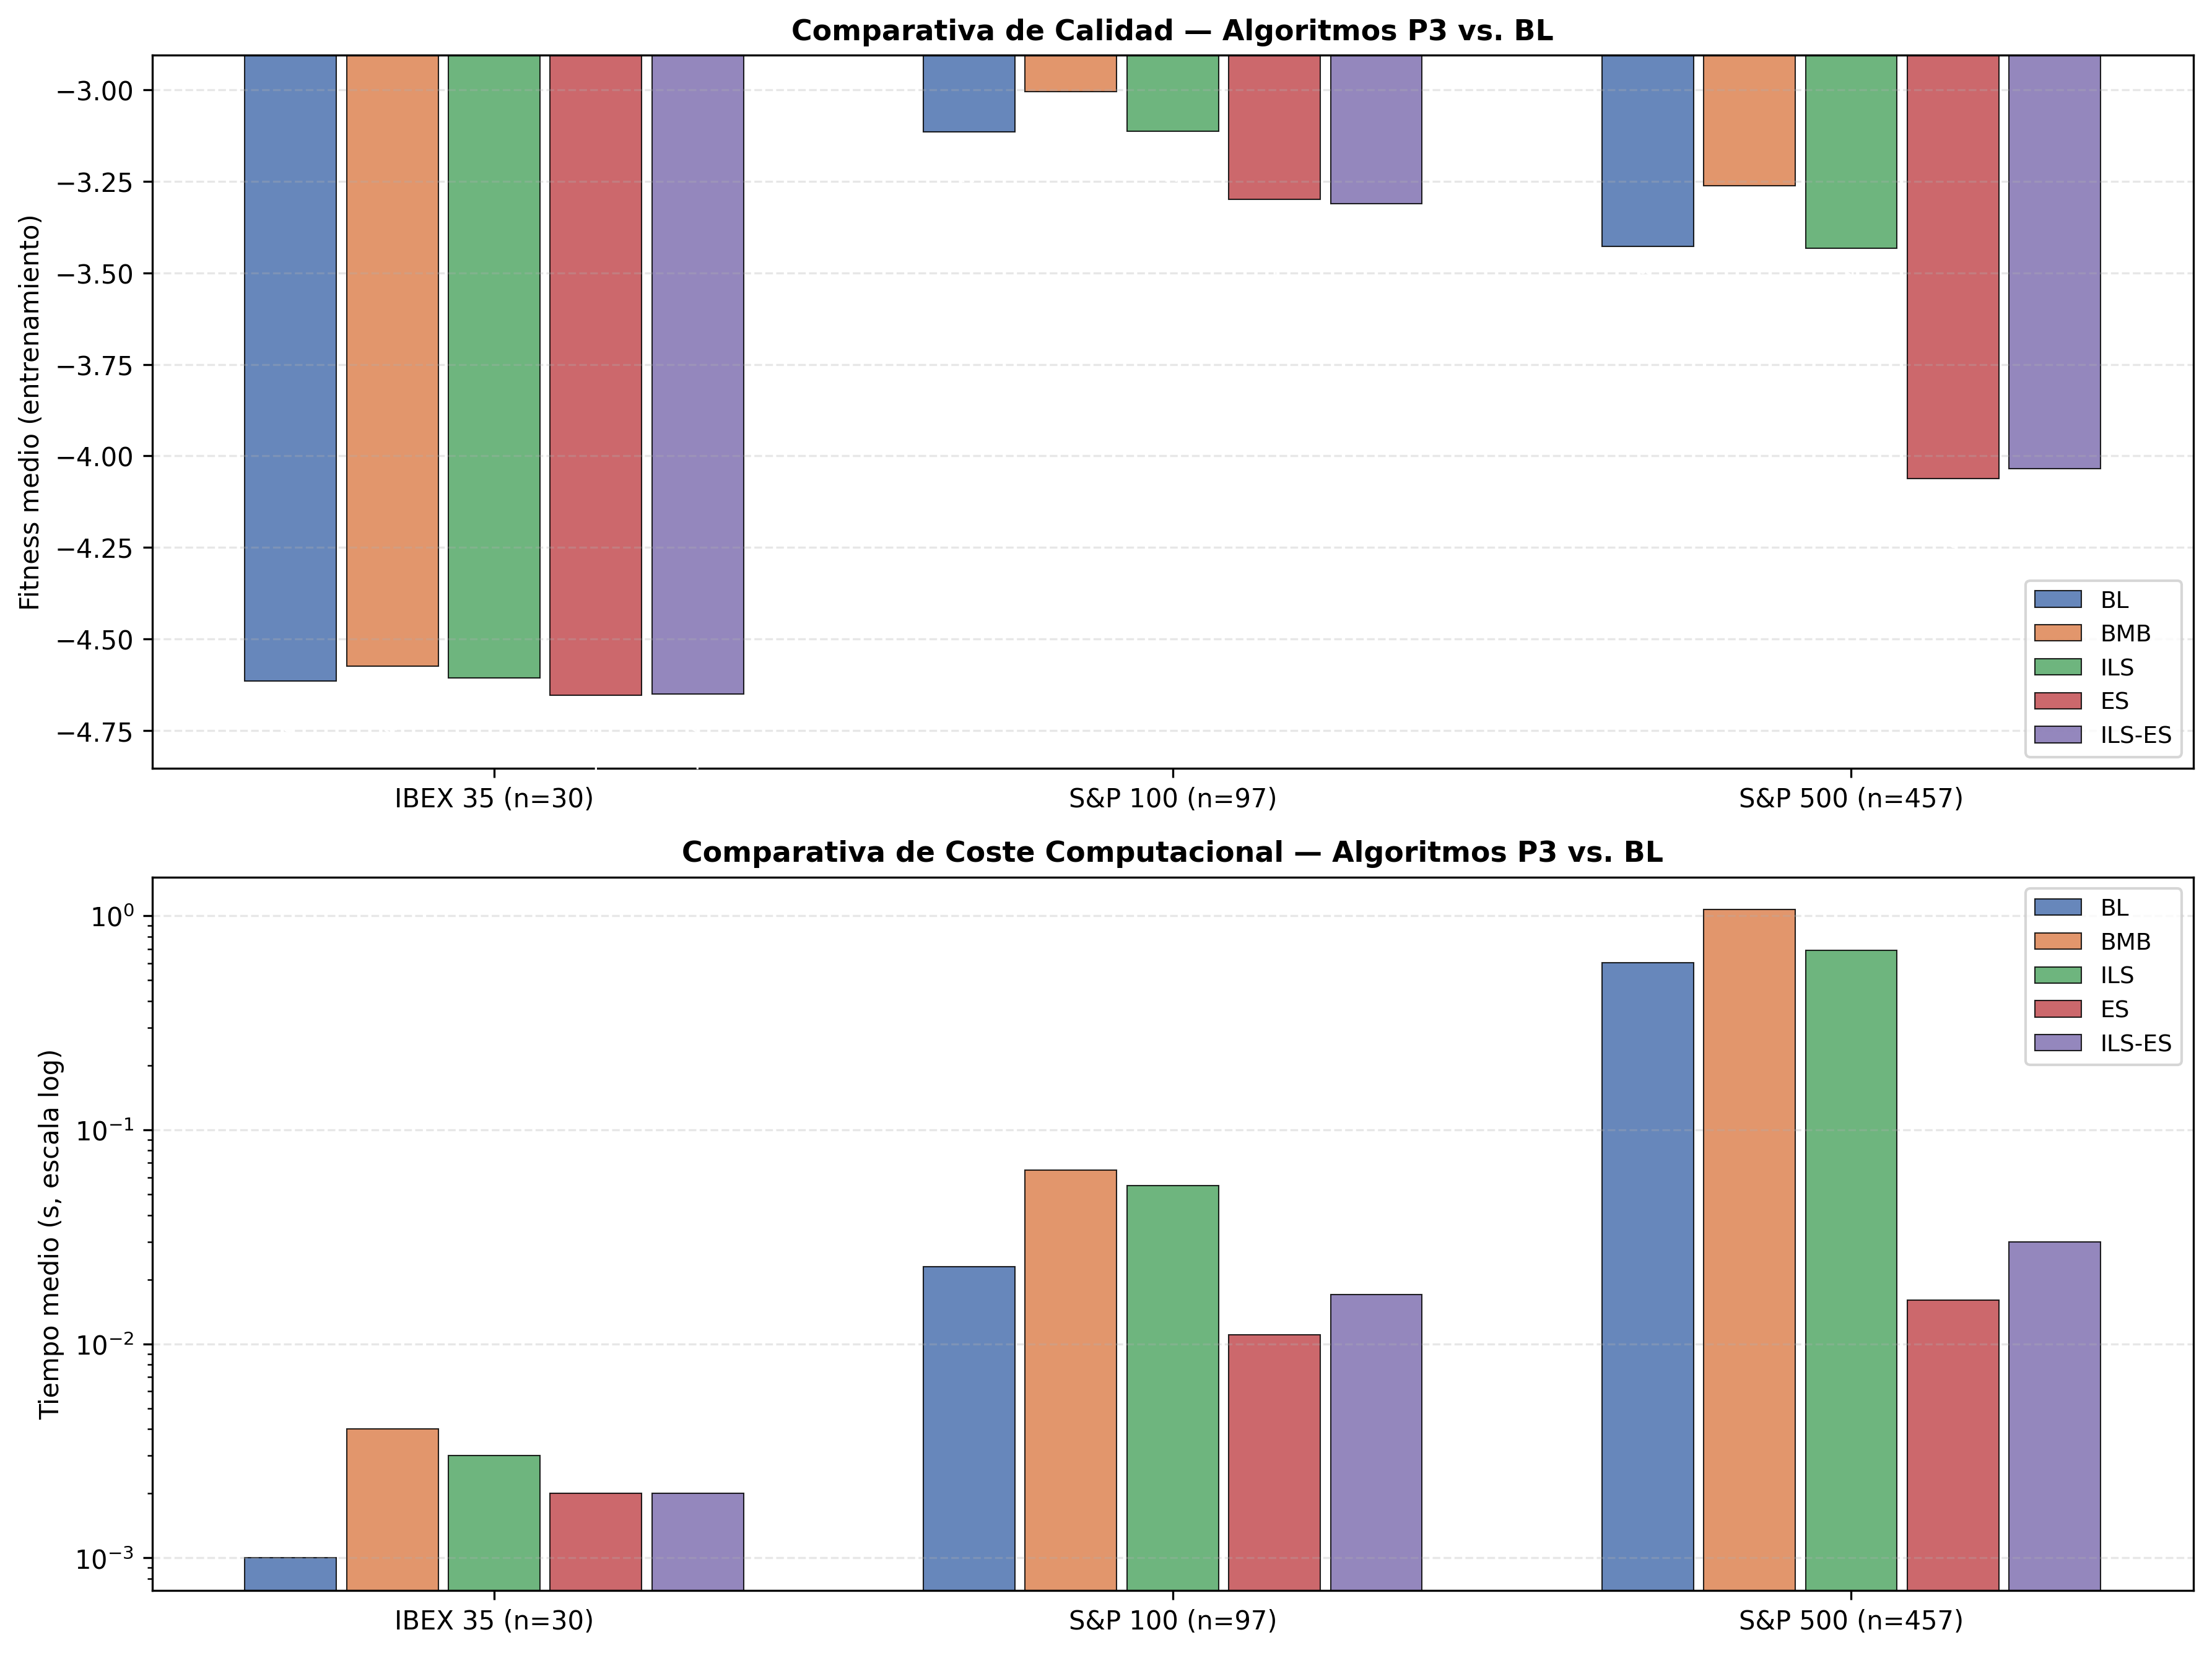
\includegraphics[width=\textwidth]{figuras/barchart_p3_comparativa.png}
\caption{Comparativa directa de fitness (arriba) y tiempo en escala logarítmica (abajo)
para los algoritmos P3 y BL en los tres mercados.}
\label{fig:barchart-p3}
\end{figure}

La Figura~\ref{fig:scatter-tradeoff} ilustra el trade-off fundamental: ES e ILS-ES ocupan
la zona de \textit{bajo tiempo y baja calidad} en S\&P 500, mientras que BMB e ILS se desplazan
hacia tiempos mayores con calidad superior. En IBEX 35, todos los algoritmos de P3 se agrupan
en la zona de bajo coste ($<0.01$ s), siendo BMB el de mayor calidad relativa.

La Figura~\ref{fig:barchart-p3} confirma en escala logarítmica que \textbf{ES e ILS-ES son
entre 3$\times$ y 40$\times$ más rápidos que BMB e ILS} en S\&P 500, pagando ese coste con
una reducción de calidad del $\approx 18\,\%$ respecto a BL. Este trade-off clásico
intensificación-coste es la razón por la que el guion incluye técnicas de trayectoria tanto
simple (ES) como múltiple (BMB, ILS): dependiendo de las restricciones de tiempo de la aplicación
real, uno u otro tipo de algoritmo resultará más adecuado.


